\documentclass[xcolor=table, handout]{beamer}

\usepackage{shyne}

% Theme settings
\setbeamertemplate{navigation symbols}{}

\usetheme{Madrid}
\usefonttheme{structurebold}

\AtBeginSection[]
{ 	\begin{frame}{}

	{
	\usebeamerfont{frametitle}
	\begin{beamercolorbox}
		[wd={\textwidth}, center, sep=.2in, rounded=true, shadow=true]
		{frametitle}
	Chapter \thesection\\  \secname 
	\end{beamercolorbox}
	}
	
	\end{frame} 
}

\AtBeginSubsection[]
{ 	\begin{frame}{}

	{
	\usebeamerfont{frametitle}
	\begin{beamercolorbox}
		[wd={\textwidth}, center, sep=.2in, rounded=true, shadow=true]
		{frametitle}
	Section \thesection .\thesubsection\\  \subsecname 
	\end{beamercolorbox}
	}
	
	\end{frame} 
}

\title[Chapter 1]{Stat 201: Statistics I\\ Week 1 }
\author[M. Shyne]{}
\institute[Metro State]{
\includegraphics[width=1.75in]{../images/metro_logo}}
\date{May 15, 2017}


\begin{document}

\frame{\titlepage}

% Chapter 1
\section{Introduction to Statistics}

% Section 1.1
\subsection{Review and Preview}

\begin{frame}
\frametitle{What is statisitcs?}

\begin{block}{}
\large \bt{Statistics} is the science of using data to learn about the world.
\end{block}

\pause

\begin{block}{}
Statistics is involved in\ldots
\begin{itemize}
\item Designing studies and experiments
\item Collecting data
\item Producing informative summaries of data
\item Analyzing data
\item Interpreting results (answering questions)
\end{itemize}
\end{block}

\end{frame}

\begin{frame}
\frametitle{Populations and samples}

\begin{block}{}
\large A \bt{population} is any group that we are interested in knowing something about.
\end{block}

\pause

\begin{block}{}
\large A \bt{census} is when data is collected from \emph{every} member of a population.
\end{block}

\pause

\begin{block}{}
\large A \bt{sample} is a subset of a population used to represent the whole population.
\end{block}

\end{frame}


\begin{frame}
\frametitle{Population and sample examples}

\begin{exampleblock}{Example}
\begin{center}
\begin{tabular}{p{1.8in} | p{1.8in} }
Population & Sample\\
\hline
The entire population of the United States & Respondents to an internet survey\\
\pause
Males over 40 who have high blood pressure & High blood pressure patients in a clinical trial\\
\pause
Students enrolled at Metro State in 2017 & You (the students in this class)\\
\pause
Statistics classes in Minnesota & The summer semester statistics classes at Metro State\\
\end{tabular}
\end{center}
\end{exampleblock}

\end{frame}

% Section 1.2
\subsection{Statistical and Critical Thinking}

\begin{frame}
\frametitle{Statistical thinking}
\begin{itemize}

\item Prepare
\begin{itemize}
\item [1] Context
\item [2] Source of the data
\item [3] Sampling method
\end{itemize}

\item Analyze
\begin{itemize}
\item [1] Graph the data
\item [2] Explore the data
\item [3] Apply statistical method
\end{itemize}

\item Conclude
\begin{itemize}
\item [1] Significance
\end{itemize}

\end{itemize}
\end{frame}

\begin{frame}
\frametitle{Prepare: Context}
\begin{block}{}
\begin{itemize}
\item What do the data mean?
\item What is the goal of the study?
\item Can the data answer the question of interest?
\end{itemize}
\end{block}

\end{frame}

\begin{frame}
\frametitle{Prepare: Source of the data}
 
\begin{block}{}
\begin{itemize}
\item Are the data from a source with a special interest so that there is pressure to obtain results that are favorable to the source?
\end{itemize} 
\end{block}

\end{frame}

\begin{frame}
\frametitle{Prepare: Sampling method}
 
\begin{block}{}
\begin{itemize}
\item Were the data collected in a way that is biased?
\end{itemize} 
\end{block}
 
\pause

\begin{block}{}
\large A \bt{voluntary response sample} (or \bt{self-selected sample}) is one in which the respondents themselves decide whether to be included. 
\end{block}
\end{frame}

\begin{frame}
\frametitle{Analyze}
 
\begin{block}{}
\begin{itemize}
\item [1] Graph the data
\item [2] Explore the data
\begin{itemize}
\item Are there any outliers?
\item What important statistics summarize the data?
\item How are the data distributed?
\item Are there missing data?
\end{itemize}
\item [3] Apply statistical method
\end{itemize}
\end{block}

\begin{block}{}
Most of the course concerns the analyze step.
\end{block}
\end{frame}

\begin{frame}
\frametitle{Conclude: Significance}

\begin{block}{}
\begin{itemize}
\item Do the results have statistical significance?
\item Do the results have practical significance?
\end{itemize}
\end{block}

\pause

\begin{exampleblock}{Example}
A clinical triel shows a new drug lowers systolic blood pressure by an average of 5 mmHg. Results are statistically significant, but may not be practically significant.
\end{exampleblock}
\end{frame}

\begin{frame}
\frametitle{Potential pitfalls: Misleading conclusions}

\begin{block}{}
Mistaking an association or relationship between two variables or factors for one factor causing the other.
\end{block}

\pause

\begin{alertblock}{!!!}
\Large Correlation does not imply causation.
\end{alertblock}

\end{frame}

\begin{frame}
\frametitle{Potential pitfalls: Reported results}

\begin{block}{}
\bt{Reported results} are data provided by the subjects of a study, rather than measured directly.
\end{block}


\end{frame}

\begin{frame}
\frametitle{Potential pitfalls: Small samples}

\begin{block}{}
Sample size is important. Be wary of results drawn from very small samples.
\end{block}


\end{frame}

\begin{frame}
\frametitle{Potential pitfalls: Loaded questions}

\begin{block}{}
\bt{Loaded questions} are those designed to elicit a particular response or to influence the subject.
\begin{itemize}
\item Also known as: push polls
\end{itemize}
\end{block}


\end{frame}

\begin{frame}
\frametitle{Potential pitfalls: Order of questions}

\begin{block}{}
The order of questions can influence responses.
\end{block}

\end{frame}

\begin{frame}
\frametitle{Potential pitfalls: Nonresponse / missing data}

\begin{block}{}
When subjects refuse to participate or data is not collected for any reason, bias can be introduced if there are characteristics shared by subjects who have missing data or those who do not.
\end{block}

\end{frame}

\begin{frame}
\frametitle{Potential pitfalls: Precise numbers}

\begin{block}{}
Precision is not the same thing as accuracy.
\end{block}

\begin{center}
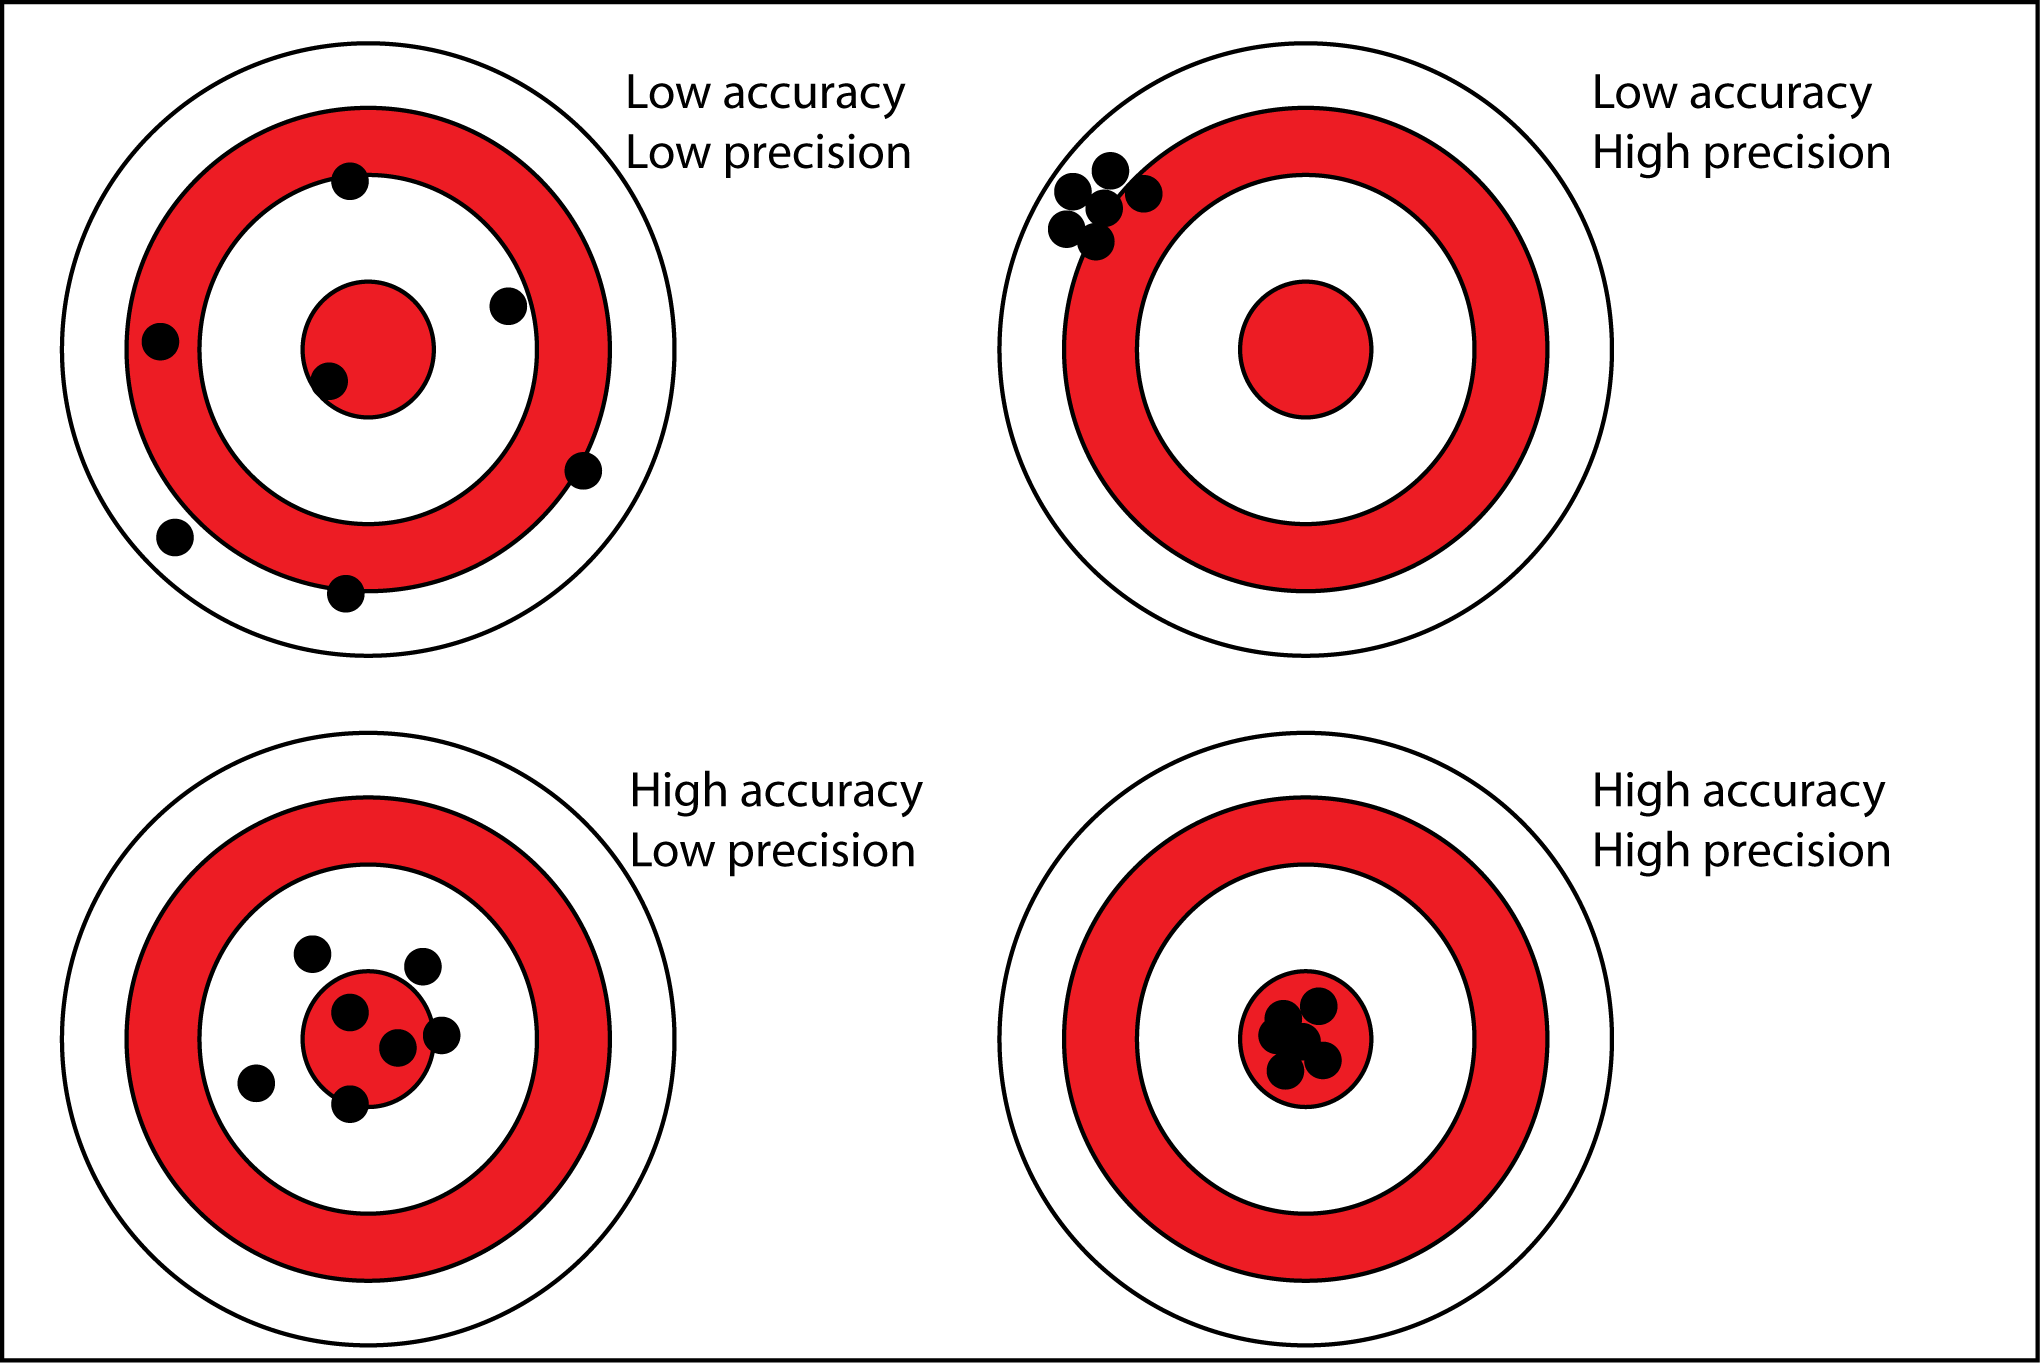
\includegraphics[width=3.5in]{../images/precision_accuracy}
\end{center}
\end{frame}

\begin{frame}
\frametitle{Potential pitfalls: Percentages}

\begin{block}{}
Sometimes percentages are used in confusing ways. Remember, 100\% of a thing is all of it. Percentages above 100, or phrases like ``a reduction of 100\%", do not always have clear meanings. 
\end{block}


\end{frame}

\begin{frame}
\frametitle{Percentages: Review}

\begin{block}{}
\begin{itemize}
\item A \bt{percentage} is number describing a proportion as an amount out of 100 (per cent).
\pause
\item We can also describe a proportion as a fraction of 1.
\[\ds \frac {50}{100} = \frac 1 2 \quad \implies \quad 50\% = .50\]
\pause
\item 100\% represents a whole, just as for proportions 1 represents a whole.
\pause
\item It often doesn't make sense to talk about percentages greater than 100\%.
\end{itemize}
\end{block}
\end{frame}

\begin{frame}
\frametitle{Percentages: Calculations}
\begin{exampleblock}{}
To convert from percentage to proportion, divide by 100:
\[56\% \quad \implies \quad \frac {56}{100} = 0.56\]
\pause
To convert from proportion to percentage, multiply by 100:
\[\frac 5 8 = 0.625 \quad \implies \quad 0.625 \times 100 = 62.5\%\]
\pause
To find the quantity a percentage represents:
\[\text{13\% of 264}\quad \implies \quad \frac {13}{100} \times 264 = 34.32\]
\pause
To find the percentage a quantity represents:
\[\text{135 out of 475} \quad \implies \quad \frac {135}{475} \times 100 = 28.42\ldots \%\]
\end{exampleblock}
\end{frame}

% Section 1.3
\subsection{Types of Data}

\begin{frame}
\frametitle{Parameters and statistics}

\begin{block}{}
\large A \bt{parameter} is a value describing an aspect of a population.
\end{block}
\pause
\begin{block}{}
\large A \bt{statistic} is a value describing an aspect of a sample.
\end{block}
\pause
\begin{exampleblock}{Example}
\begin{itemize}
\item The average height of adult men in the U.S. is 72 inches: \bt{Parameter}

\item The average height of 30 randomly selected male Metro State students is 68.5 inches: \bt{Statistic}
\end{itemize}
\end{exampleblock}

\end{frame}

\begin{frame}
\frametitle{Types of data}

\begin{block}{}
\large \bt{Quantitative} data are numbers representing amounts, sizes, time or other measurements.\\
Also known as: Numeric
\end{block}

\begin{exampleblock}{Example}
Class size, height, age, systolic blood pressure, temperature
\end{exampleblock}

\pause

\begin{block}{}
\large \bt{Categorical} data are values representing groups or categories.
\begin{itemize}
\item Also known as: qualitative, attribute
\end{itemize}
\end{block}

\begin{exampleblock}{Example}
Gender, state of residence, football player's numbers, pain scale
\end{exampleblock}

\end{frame}

\begin{frame}{Types of data: Quantitative}
\begin{block}{}
\large \bt{Discrete} data have a finite number of possible values. There are gaps in the possible values.
\end{block}

\begin{exampleblock}{Example}
Class size: can't have a class size of 22.5
\end{exampleblock}
\pause
\begin{block}{}
\large \bt{Continuous} data have an infinite number of possible values. There are no gaps in possible values.
\end{block}

\begin{exampleblock}{Example}
Height: a height of 70.2641... inches is possible (not necessarily useful, but possible)
\end{exampleblock}

\end{frame}

\begin{frame}
\frametitle{Levels of measurement: Nominal}
\begin{block}{}
\large The \bt{nominal} level of measurement is categorical data that are names or labels for groups or categories. There is no reasonable order or ranking to the categories.
\end{block}
\pause
\begin{exampleblock}{Example}
\begin{itemize}
\item Gender: \emph{male} or \emph{female}
\item State of residence: \emph{Minnesota}, \emph{Wisconsin}, etc.
\end{itemize}
\end{exampleblock}
\pause
\begin{alertblock}{Hint}
The root word \emph{nom} means ``name''.
\end{alertblock}
\end{frame}

\begin{frame}
\frametitle{Levels of measurement: Ordinal}
\begin{block}{}
The \bt{ordinal} level of measure is categorical data that are naturally ordered or ranked.
\end{block}
\pause
\begin{exampleblock}{Example}
\begin{itemize}
\item Pain scale: \emph{No pain} $<$ \emph{Moderate pain} $<$ \emph{Heavy pain}
\item Grades: \emph A $>$ \emph B $>$ \emph C $>$ \emph D $>$ \emph F
\end{itemize}
\end{exampleblock}
\end{frame}

\begin{frame}
\frametitle{Levels of measurement: Interval}
\begin{block}{}
\large The \bt{interval} level of measurement is quantitative data where\\ the difference between values has meaning but where there is no natural ``zero''.
\end{block}
\pause
\begin{exampleblock}{Example}
\begin{itemize}
\item Temperature: The difference between 101\textdegree F and 98.6\textdegree F is meaningful, but 0\textdegree F does not mean no temperature.
\item Year: 2017 is four years after 2013, but year 0 does not mean no years.
\end{itemize}
\end{exampleblock}
\end{frame}

\begin{frame}
\frametitle{Levels of measurement: Ratio}
\begin{block}{}
\large The \bt{ratio} level of measurement is quantitative data where the difference between values and relative sizes of values have meaning. There is a natural ``zero''.
\end{block}
\pause
\begin{exampleblock}{Example}
\begin{itemize}
\item Age: Someone who is 40 years old is \emph{twice} as old as someone who is 20 years old. Zero does mean no age.

\item Height: A tree that is 10 feet tall is \emph{one third} as tall as a tree that is 30 feet tall. Zero does mean no height.
\end{itemize}

\end{exampleblock}
\end{frame}

% Section 1.4
\subsection{Collecting Sample Data}

\begin{frame}
\frametitle{Samples}

\begin{block}{}
\begin{itemize}
\item Remember: When we want to know something about a population and we can't collect data from the entire population, we can collect data from a subset, or a \bt{sample}, of the population instead.
\pause
\item We can then use statistics to learn something about the whole population.
\pause
\item Therefore, how we pick our sample is very important in how valid the interpretation of our results are.
\end{itemize}
\end{block}
\pause
\begin{exampleblock}{Example}
\begin{itemize}
\item Suppose we are collecting data for the Metro State Annual Taco Survey (MSATS). It would be difficult, if not impossible, to ask every student about their taco eating habits. We need a sample.
\end{itemize}
\end{exampleblock}
\end{frame}

\begin{frame}
\frametitle{Types of samples: Random sample}

\begin{block}{}
\large A \bt{random sample} is a sample selected such that every individual member of a population has an equal chance of being included.
\end{block}
\pause
\begin{block}{}
\large A \bt{simple random sample} is a sample selected such that every possible sample of a specific size has an equal chance of being selected.
\begin{itemize}
\item These are the ``best" kind of samples for producing valid, unbiased results, but they are not always easy to get. 
\end{itemize}
\end{block}
\pause
\begin{exampleblock}{Example}
\begin{itemize}
\item Given an alphabetical list of students, use a random number generator to select a sample.
\end{itemize}
\end{exampleblock}

\end{frame}

\begin{frame}
\frametitle{Types of samples: Systematic sampling}

\begin{block}{}
\large \bt{Systematic sampling} is a method where every $k$th member of of a population is selected.
\begin{itemize}
\item These samples are ofter easier to produce, but can lead to biased samples. 
\end{itemize}
\end{block}
\pause
\begin{exampleblock}{Example}
\begin{itemize}
\item Given an alphabetical list of students, select every fifth student until you have a sample of the desired size.
\end{itemize}
\end{exampleblock}

\end{frame}

\begin{frame}
\frametitle{Types of samples: Convenience sampling}

\begin{block}{}
\large \bt{Convenience sampling} is a method of choosing members of a population that are nearby or easy to access.
\begin{itemize}
\item The easiest of all methods, but by far the lowest quality data for producing results.
\end{itemize}
\end{block}
\pause
\begin{exampleblock}{Example}
\begin{itemize}
\item Wander the halls before class, asking students who happen to walk by.
\item Put a poll on the Metro State website.
\end{itemize}

\end{exampleblock}
\end{frame}

\begin{frame}
\frametitle{Types of samples: Stratified sampling}

\begin{block}{}
\large \bt{Stratified sampling} is a method where the population is divided into groups and samples are selected from each group.
\begin{itemize}
\item Useful when you want to ensure that a factor of interest has enough representation, but it is not a random sample as we have defined it.
\end{itemize}
\end{block}
\pause
\begin{exampleblock}{Example}
\begin{itemize}
\item If we have particular interest in the taco consuming difference between graduate students and undergrads, select a sample from each group.
\end{itemize}
\end{exampleblock}
\end{frame}

\begin{frame}
\frametitle{Types of samples: Cluster sampling}

\begin{block}{}
\large \bt{Cluster sampling} is a method where the population is divided into sections or clusters. Then, a number of clusters are randomly selected and all members of the clusters are included in the sample.
\begin{itemize}
\item More convenient than some methods, but better randomization the pure convenience sampling.
\end{itemize}
\end{block}
\pause
\begin{exampleblock}{Example}
\begin{itemize}
\item Choose 5 random classes, and survey all the students in those classes.
\end{itemize}
\end{exampleblock}
\end{frame}

\begin{frame}
\frametitle{Types of samples: Multistage sampling}

\begin{block}{}
\large \bt{Multistage sampling} is a when a combination of methods are used to produce a sample.
\end{block}
\pause
\begin{exampleblock}{Example}
\begin{itemize}
\item Choose random classes by cluster sampling, and then take a simple random sample of students from each chosen class.  
\end{itemize}
\end{exampleblock}
\end{frame}

\begin{frame}
\frametitle{Types of studies}

\begin{block}{}
\large In an \bt{observational study} data is collected from a sample without trying to modify behavior or results. 
\end{block}
\pause
\begin{block}{}
\large In an \bt{experiment} a change (treatment) is made to some or all of sample and then data is collected in order to detect changes. 
\end{block}

\end{frame}

\begin{frame}
\frametitle{Types of observational studies}

\begin{block}{}
A \bt{cross-sectional} study measures and collects data from one point in time (the present).
\end{block}
\pause
\begin{block}{}
A \bt{retrospective} study collects data from the past, whether from recollections or by examining records.
\begin{itemize}
\item Also know as: case-control
\end{itemize}
\end{block}
\pause
\begin{block}{}
A \bt{prospective} study follows subjects into the future to measure and collect data.
\begin{itemize}
\item Also know as: longitudinal study, cohort study
\end{itemize}
\end{block}
\end{frame}


% Chapter 2
\section{Summarizing and Graphing Data}

% Section 2.2
\addtocounter{subsection}{1}
\subsection{Frequency Distributions}

\begin{frame}
\frametitle{Frequency distributions}

\begin{block}{}
A \bt{frequency} is the number of times a particular value occurs in a set of data, i.e. the count.
\end{block}
\pause
\begin{block}{}
A \bt{frequency distribution} (or \bt{frequency table}) summarizes a set of data by listing the frequencies of data in categories or classes (groups).
\begin{itemize}
\item For categorical data, the categories are simply the possible values of the data.
\item For quantitative data, the classes are usually ranges of possible values.
\end{itemize}
\end{block}
\end{frame}

\begin{frame}
\frametitle{Frequency distribution for categorical data}

\begin{exampleblock}{Example}
\bt{Favorite kind of taco} = \{Chicken, Fish, Fish, Veggie, Chicken, Beef \}

\begin{center}
\begin{tabular}{c | c}
Kind of taco & Frequency\\
\hline
Beef & 1\\
Chicken & 2\\
Pork & 0\\
Fish & 2\\
Veggie & 1
\end{tabular}
\end{center}
\end{exampleblock}

\end{frame}

\begin{frame}
\frametitle{Frequency distribution for quantitative data}

\begin{exampleblock}{Example}
\bt{Tacos eaten} = \{3, 0, 17, 6, 4, 3, 5 \}

\begin{center}
\begin{tabular}{c | c}
Number of tacos eaten & Frequency\\
\hline
0 - 4 & 4\\
5 - 9 & 2\\
10 - 14 & 0\\
15 -20 & 1
\end{tabular}
\end{center}
\end{exampleblock}

\end{frame}

\begin{frame}
\frametitle{Relative frequency}

\begin{block}{}
\bt{Relative frequency} is the proportion (fraction) of the whole data set that resides in each category or class. When expressed as a percent it is called \bt{percentage frequency}.
\end{block}
\pause
\begin{block}{}
To calculate: For each class,
\[\text{Relative frequency} = \frac{\text{class frequency}}{\text{total count}}\]
\[\text{Percentage frequency} = \frac{\text{class frequency}}{\text{total count}} \times 100\]
\end{block}

\end{frame}

\begin{frame}
\frametitle{Relative frequency example}

\begin{exampleblock}{Example}

\begin{center}
\begin{tabular}{c | c | c | c}
Tacos eaten & Frequency & Relative & Percentage\\
\hline
0 - 4 & 4 & 0.5714 & 57.14 \%\\
5 - 9 & 2 & 0.2857 & 28.57 \%\\
10 - 14 & 0 & 0 & 0 \%\\
15 -20 & 1 & 0.1428 & 14.28 \%\\
\hline
Total & 7 & 1 & 100 \%
\end{tabular}
\end{center}
\end{exampleblock}

\end{frame}

\begin{frame}
\frametitle{Cumulative frequency}

\begin{block}{}
\bt{Cumulative frequency} is the frequency for a class and \emph{all previous classes}.
\end{block}
\pause
\begin{exampleblock}{Example}

\begin{center}
\begin{tabular}{c | c | c }
Tacos eaten & Frequency & Cumulative\\
\hline
0 - 4 & 4 & 4\\
5 - 9 & 2 & 6\\
10 - 14 & 0 & 6\\
15 -20 & 1 & 7\\
\end{tabular}
\end{center}
\end{exampleblock}

\end{frame}

\begin{frame}
\frametitle{Normal distributions}

\begin{block}{}
A \bt{normal distribution} can be identified from a frequency table that has the following characteristics:
\begin{itemize}
\item The frequencies start low, increase to a high point and then decrease to low frequencies at the end
\item The frequencies are approximately symmetric around the high point.
\end{itemize}
\end{block}
\end{frame}

\begin{frame}
\frametitle{Normal distributions, example}

\begin{exampleblock}{Example}
\begin{columns}[c]
\column{.5\textwidth}
\begin{center}
\begin{tabular}{c|c}
\multicolumn{2}{c}{\emph{Normal}}\\
IQ & Frequency\\
\hline
80 - 89 & 1 \\
90 - 99 &  5\\
100 - 109 & 11\\
110 - 119 & 10\\
120 - 129 &  4\\
130 - 139 & 2

\end{tabular}
\end{center}
\column{.5\textwidth}
\begin{center}
\begin{tabular}{c|c}
\multicolumn{2}{c}{\emph{Not normal}}\\
IQ & Frequency\\
\hline
80 - 89 & 2\\
90 - 99 &  9 \\
100 - 109 &  13\\
110 - 119 & 4 \\
120 - 129 & 3\\
130 - 139 & 1

\end{tabular}
\end{center}

\end{columns}


\end{exampleblock}

\end{frame}

\begin{frame}
\frametitle{Gaps in frequency tables}
\begin{block}{}
A \bt{gap} of frequencies in a table indicates that the data probably come from two different populations.
\end{block}
\pause
\begin{block}{}
The converse is not necessarily true. Data from two different populations might not display a gap.
\end{block}
\pause
\begin{exampleblock}{Example}
\begin{itemize}
\item Pennies made before 1983 are 95\% copper and 5\% zinc.
\item Pennies made after 1983 are 2.5\% copper and 97.5\% zinc. 
\end{itemize}
\end{exampleblock}
\end{frame}

\begin{frame}{Gaps in frequency tables, example}

\begin{exampleblock}{Example, cont.}
\begin{center}
\begin{tabular}{c|c}
Weight (g) of penny & Frequency\\
\hline
2.40 - 2.49 & 18 \\
2.50 - 2.59 & 19\\
2.60 - 2.69 & 0\\
2.70 - 2.79 & 0\\
2.80 - 2.89 & 0\\
2.90 - 2.99 & 2\\
3.00 - 3.09 & 25\\
3.10 - 3.19 & 8\\
\end{tabular}
\end{center}
\end{exampleblock}
\end{frame}


\end{document}